\documentclass[11pt]{standalone}
\usepackage[usenames]{color} %used for font color
\usepackage{amssymb} %maths
\usepackage{amsmath} %maths

\usepackage[no-math]{fontspec}
\usepackage{unicode-math}
\setmainfont{Lato}
\setmathfont{Stix Two Math}

\usepackage{pgf,xcolor}
\definecolor{itwm_blue_04}{HTML}{005A94}
\definecolor{itwm_red}{HTML}{C00000}
\definecolor{itwm_yellow}{HTML}{FFEC7F}

\usepackage{tikz}
\usetikzlibrary{shapes.misc, shadows, decorations}
\usetikzlibrary{positioning, arrows}
\usetikzlibrary{backgrounds}
\usetikzlibrary{calc}
\usepackage{pgfplots}
\pgfplotsset{compat=newest}
\usepgfplotslibrary{fillbetween}
\usepackage{tikzpagenodes}
\usetikzlibrary{patterns}


\begin{document}
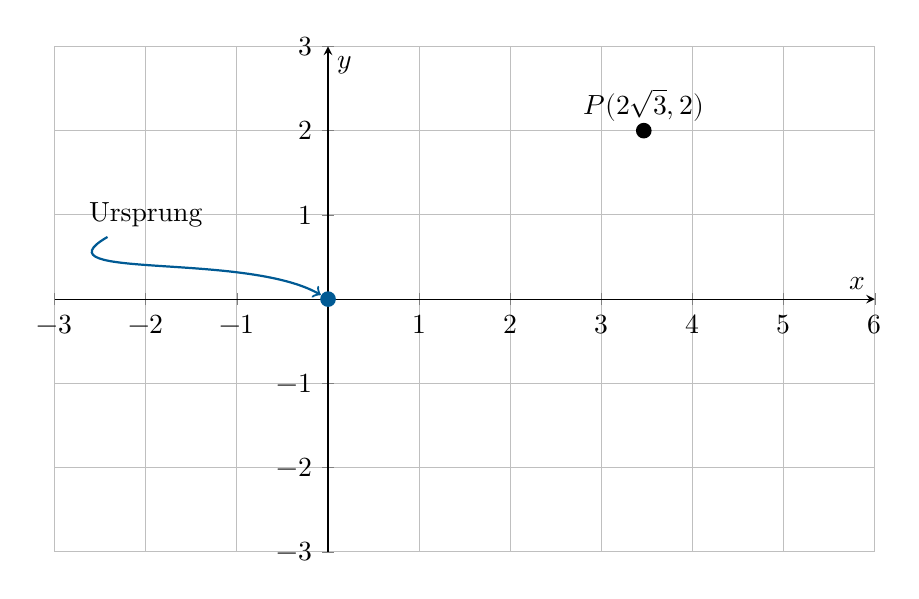
\begin{tikzpicture}
\begin{axis}[
    domain=-3:6,
    axis lines = center,
    xlabel = {$x$},
    ylabel = {$y$},
    height=8cm, width=12cm, 
    xmin=-3, xmax=6, ymin=-3, ymax=3,
    xtick={-3,-2,...,6},
    ytick={-3,-2,...,3},
    grid = both
]
\node[fill, black, circle, inner sep=-2] at (3.4641,2) {};
\node[above] at (3.4641,2) (point) {$P(2\sqrt{3},2)$};
\node[itwm_blue_04, fill, circle, inner sep=-2] (ursprung) at (0,0) {};
\node (labelursprung) at (-2,1) {Ursprung};
\draw[->, thick, itwm_blue_04] (labelursprung) to[out=-150,in=150] (ursprung);
\end{axis}
\end{tikzpicture}
\end{document}

